\documentclass[11pt]{article}

\usepackage{sbc-template}
\usepackage{graphicx} %package to manage images
\usepackage{amsmath}
\usepackage{graphicx,url}
\usepackage{mathtools}
\usepackage{blkarray, bigstrut}
\usepackage{amsmath}

\usepackage[english]{babel}   
%\usepackage[latin1]{inputenc}  
\usepackage[utf8]{inputenc}  
% UTF-8 encoding is recommended by ShareLaTex
\usepackage{verbatim}
\usepackage{listings}
\usepackage{xcolor}

\definecolor{verde}{rgb}{0,0.5,0}

%para customizar o código (ver https://en.wikibooks.org/wiki/LaTeX/Source_Code_Listings)
\lstset{language=eng, %defina a linguagem usada no trabalho
              belowcaptionskip=1\baselineskip,
                breaklines=true,
                frame=false,
                xleftmargin=\parindent,
                showstringspaces=false,
                basicstyle=\footnotesize\ttfamily,
                keywordstyle=\bfseries\color{green!40!black},
                commentstyle=\itshape\color{purple!40!black},
                identifierstyle=\color{blue},
                stringstyle=\color{orange},
                numbers=left,
            }

\sloppy

\title{Laboratoire Hubert Curien\\ Faculté des sciences et techniques\\\phantom\\ \\ Internship Summary Report}

\author{Arunava MAULIK}


\address{
  \email{arunava.maulik@etu.univ-st-etienne.fr}}


\begin{document} 

\maketitle



\section{Introduction}\phantom

This report is a brief summary of the internship topic 'Majority Vote as a source of Additional Knowledge for Classification'

\section{PROBLEM UNDERSTANDING}\phantom 

The goal of the research topic is to efficiently handle the problem of prediction on sparse data by incorporating knowledge of a domain expert.
Datasets with a large number of features and small number of training examples are quite common these days. Performing predictions on this kind of data is hugely problematic. A practical example could be a dataset with details of a rare form of disease. There would be quite a large number of features describing the disease but only a handful of samples to work with. Also, obtaining more samples would be virtually impossible.
This is where the knowledge of domain experts comes in.
Knowledge elicitation is done with the help of a probabilistic inference process and a query algorithm is devised for fast and efficient interaction with the expert. The expert usually has knowledge of the relevance of the features of the dataset or the values of certain regression coefficients which can be incorporated in the prediction model.

\section{PAC-Bayesian Bounds }\phantom

A PAC Bayesian approach is used which is well suited to the majority vote model. It is assumed that there is a normal distribution P on the classifiers, called the apriori. A posterior distribution Q is learnt using the training data which has peaks over the classifiers which perform well on this training data. The true risk associated with a stochastic classifier, which is called the Gibbs classifier, can be obtained by the empirical risk and the Kullbeck-Liebler divergence between the two distributions. The risk of the majority vote classifier is upper bounded by twice the risk of the Gibbs classifier.However, the community of classifiers tend to compensate the individual errors of the classifiers. This dramatically reduces the risk of the majority vote classifier and it is much lower than the upper bound, rendering it meaningless.\\Thus a new bound called the C-bound is introduced which is much tighter and captures this compensation. The margin of the majority vote classifier is assumed to be a random variable. \\
For all purposes, we have made 2 assumptions.
\begin{enumerate}
\item The hypothesis space is auto-complemented 
\item The distribution on this H space is quasi-uniform
\end{enumerate}

\hspace{-13mm}The C-bound is given by the following formula. We consider the first and the second moments ie, the mean and the variance of this variable for the formulation of the C-bound.
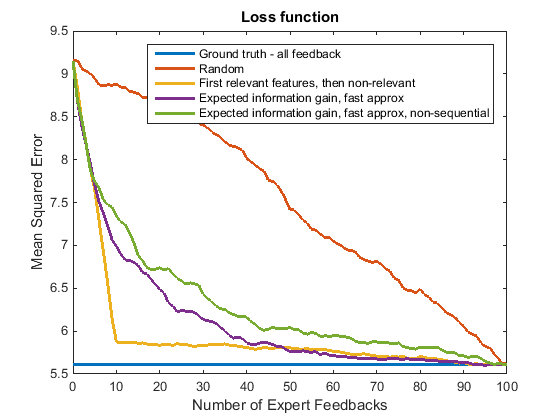
\includegraphics[width=\textwidth]{1.PNG}


\hspace{-14mm}There are a few problems with this bound.\\
\begin{enumerate}
\item This bound is on the true distribution and it can only be empirically estimated.Thus, the minimization of this bound can lead to overfitting problems.
\item As we see, the C-bound is dependant on the square of the first moment and the variance of the distribution. Usually, these are very close to 0, the quotient can lead to numerical instability.
\item This bound depends on th/e empirical estimate of the bound and the kullbeck-liebler divergence between the apriori and the posterior distribution. This KL divergence seems to be a poor regularizer and it would be best if we could get rid of this term in the C-bound.
\end{enumerate}

\hspace{-13mm}This gives rise to the MinCq algorithm which tries to take care of the above problems and finds the best quasi-uniform distribution which has an empirical margin exactly equal to $\mu$ and minimizes the variance term in the C-bound thereby minimizing the overall C-bound.\\
This algorithm can be seen as a constrained optimization problem and can be solved using quadratic programming. The CQboost algorithm is an extension of this algorithm with relaxed constraints.

\hspace{-14mm}\includegraphics[width=\textwidth]{2.PNG}

\section{Knowledge Elicitation}
This section deals with the process of systematically eliciting the knowledge of the experts using active learning where the most important features are queried about to the user first, thereby increasing information gain from each feedback and minimizing the total number of feedbacks. As opposed to the prior elicitation method where the knowledge of the experts is used to construct the apriori and later use them for learning, this method relies on interactive integration of the expert knowledge in the training itself. The first step is to calculate the posterior distribution given the observations. This posterior is sequentially updated using the feedbacks from the user(expert in this case). The query algorithm ranks the features to be asked to the expert on the basis of maximum information gain. In other words, we look to minimize the KL divergence between the present posterior distribution and the one with the new feedback thereby maximizing the information gain. \\
A sparse regression Model is used for the knowledge elicitation process.\\ Two feedback models are considered for the purpose.
\begin{enumerate}
\item Here we assume that the expert has knowledge about the values of the coefficients of the features
\item Here we assume that the expert has knowledge about the relevance of the features, 0 for not-relevant and 1 for relevant. Since the answer the answer will a 0 or 1 in every case, a  Bernoulli distribution is assumed on the features. We also take into account the confidence with which the expert shares this knowledge.
\end{enumerate}
A spike and slab sparsity inducing prior is assumed on the regression coefficients and Expectation Propagation is used to approximate this prior which consists of 2 things 
\begin{enumerate}
\item Kalman Filtering : This algorithm uses a series of measurements over time and produces estimates of unknown variables that tend to be more accurate than those based on a single measurement.
\item  Belief Propagation : This algorithm is used for inference on graphical models such as the Bayesian Network.
\end{enumerate}
Two test cases were used, 
\begin{enumerate}
\item Random selection of features to ask the expert
\item The most relevant features were queries first. 
\end{enumerate}
The MSE values for both cases are documented and it is clear that the sequentially queried algorithm performs better from start to finish. Whereas in the random feature selection, the performance drops significantly in higher dimensions, in the sequential case the performance is acceptable.The same was observed on the two datasets used for testing ie, the Amazon dataset and the Yelp dataset.\\
The next idea was to compare the results of randomly obtaining more training samples for a dataset vs adding samples which maximized the expected information gain(using active selection). \\ 
Unsurprisingly, the addition of relevant samples coupled with the sequential model for feature selection performed much better than random sample addition.

\section{Conclusion}
The PAC-Bayesian approach was used for the majority vote model and consequently the MinCq algorithm(and later CQBoost) for risk bound minimization was formulated as a quadratic program. It is free from the KL divergence which makes it somewhat immune to overfitting.\\ Also, a knowledge elicitation model where an expert/ a pool of experts are systematically queried about the co-efficients of the /relevance of features was developed for doing prediction on sparse dataset. It was observed that this model fares better than the prior elicitation model and even for rather weak feedback on the relevance of features, it fared better than random feature selection. It was also observed that obtaining more samples using active selection technique coupled with sequentially querying the expert about the relevance of features lead to much better results than randomly adding more samples.


\end{document}
